\section{Strong NP-completeness}
\label{sec:hardness}

The approximation algorithms exploit planar structure, but exact
optimization remains hard. We first state the decision and source
problems and the graph terminology used by both reductions.

\begin{definition}[Complexity and reductions]\label{def:complexity}
A \emph{polynomial-time many-one reduction} maps instances of one
decision problem to another in polynomial time, so an input is a
yes-instance if and only if its image is a yes-instance.

A decision problem is in \emph{NP} if every yes-instance has a
certificate of polynomial encoding length whose validity is
checkable in polynomial time, and no certificate is accepted on a
no-instance. It is \emph{NP-hard} if every problem
in NP admits such a reduction to it, and \emph{NP-complete} if it
is both NP-hard and in NP.
A numerical problem is \emph{strongly NP-hard} if hardness persists
when its integer data are bounded by a fixed polynomial in the
combinatorial instance size; it is \emph{strongly NP-complete} if
it is also in NP. For rational data, our restricted instances
explicitly bound both numerators and denominators.
\end{definition}

\begin{definition}[3-Partition]\label{def:three-partition}
The input consists of positive integers $a_1,\ldots,a_m,B$, where
$m=3p$ for a positive integer $p$, satisfying
\[
 s=\sum_{i=1}^m a_i=pB,\qquad B/4<a_i<B/2.
\]
The question is whether $[m]$ can be partitioned into $p$ groups
$I_1,\ldots,I_p$ with $|I_b|=3$ and
$\sum_{i\in I_b}a_i=B$ for every $b$.
\end{definition}

\begin{symboltable}
$m=3p,\ [m]$ & Number of source items and their index set.\\
$a_i,\ B$ & Item size $i$ and target sum of each bin.\\
$s=pB=\sum_i a_i$ & Total item size and total capacity of the $p$ bins.\\
$I_b$ & Index set of the three items assigned to source bin $b$.\\
\end{symboltable}

Both reductions use the strong NP-completeness of this
problem~\cite{gj1979}.
We use the NP-hard restriction in which $B$ is polynomially bounded
in $m$. The case $p=1$ is a trivial yes-instance, so excluding it
preserves NP-hardness. In this restriction each $a_i$ is
polynomially bounded, so the explicit
repetitions in our constructions remain polynomial in the source
size. A partition into $p$ groups of sum $B$
then necessarily has three items per group: two items sum to less
than $B$, while four items sum to more than $B$.

\begin{definition}[Paths and matchings]\label{def:paths-and-matchings}
A \emph{path} is an undirected graph with distinct vertices
$v_0,\ldots,v_k$ and edges exactly
$\{v_{j-1},v_j\}$ for $1\le j\le k$.
A \emph{linear forest} is a disjoint union of paths, allowing
isolated vertices. Throughout, an \emph{odd path} has an odd number
of vertices; when its edge count matters, we state that count
explicitly. Positions are numbered locally from zero along each item
path, separately from global hypothesis indices.

A \emph{matching} is a set of edges with no shared endpoint.
A vertex is \emph{unmatched} if it is incident to no chosen edge.
A \emph{maximum matching} has the largest possible number of edges.
A \emph{perfect matching} leaves no vertex unmatched.
\end{definition}

Both reductions turn the same source decision into a choice of one bin
for each item. To represent those choices, we place an item on an odd
path and supply tests for each vertex and each adjacent pair. The
distinguished hypothesis forces an optimal tree to use a maximum
matching of these pair tests; by Lemma~\ref{lem:odd-path}, the one
unmatched even-position vertex then specifies the item's bin. This
Each unmatched-position choice changes a different statistic. For
maximum depth, clouds change the number of branches at each height;
for expected depth, weights change the pair-mass histogram. Summing
these statistics across the items recovers the source bin loads.
Finally, the parabola realizes every singleton and adjacent-pair test
as a supplied line, and the cloud replacement in
Section~\ref{sec:uniform-hardness} transfers the weighted expected-depth
instance to a uniform prior while adding the same fixed internal cost
to every maximum matching.

\subsection{The geometric realization and the matching choice}

For integer abscissae, the line
\[
 I_{a,b}:\quad
 4y-4(a+b)x+(2a-1)(2b+1)=0
\]
has value $4(x-a+\tfrac12)(x-b-\tfrac12)$ on $(x,x^2)$.
Its negative answer selects exactly the integer abscissae
$a,\ldots,b$. This realizes interval membership using one line.
The line
\begin{equation}\label{eq:private-singleton}
 P_t:\quad 2y-4tx+2t^2-1=0
\end{equation}
has value $2(x-t)^2-1$, and its negative answer isolates exactly
the point of abscissa $t$. Both formulas are nonzero at all integer
abscissae, so every answer is binary.
The tangent $y=2tx-t^2$ exposes the point $(t,t^2)$, since every
other parabola point lies strictly above it. The constructed
hypotheses are therefore in strictly convex position.

We use the negative answer class of each displayed line as its
membership set. Consequently, a hit in
Definition~\ref{def:membership-spine} is precisely a negative affine
sign, while the distinguished hypothesis is placed outside every such
set. This convention lets the combinatorial path tests above enter the
membership-spine framework without changing the supplied queries.



With this membership convention, the two formulas realize every
singleton and adjacent-pair test used by the matching construction.
The parabola keeps all hypotheses exposed on the convex hull, and the
integer abscissae give explicit integer coefficients for each line.
Figure~\ref{fig:parabola-queries} illustrates $I_{2,5}$ and $P_4$ on
the points with integer abscissae from $0$ to $8$.

\begin{figure}[tbp]
\centering
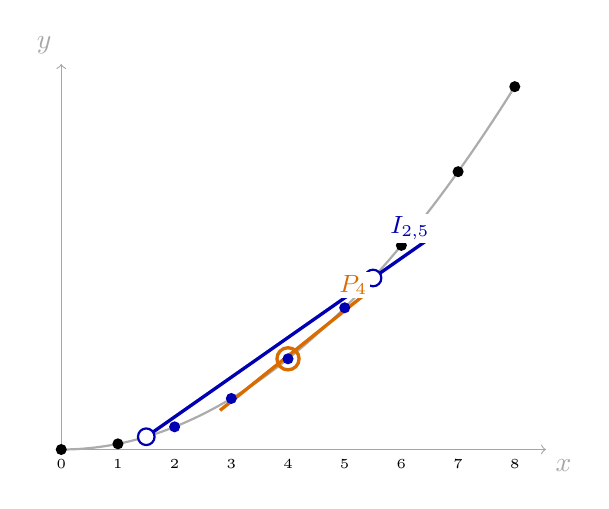
\begin{tikzpicture}[x=0.72cm,y=0.072cm]
  \draw[->,gray!70] (0,0)--(8.55,0) node[below right] {$x$};
  \draw[->,gray!70] (0,0)--(0,68) node[above left] {$y$};
  \foreach \x in {0,...,8} {
    \node[below,font=\tiny] at (\x,0) {\x};
  }
  \draw[thick,gray!65] plot[domain=0:8,samples=81] (\x,{(\x)^2});
  \draw[very thick,blue!70!black]
    plot[domain=1.5:6.5,samples=60] (\x,{7*\x-8.25});
  \draw[very thick,orange!85!black]
    plot[domain=2.8:5.4,samples=50] (\x,{8*\x-15.5});
  \draw[blue!70!black,fill=white,thick] (1.5,2.25) circle (3pt);
  \draw[blue!70!black,fill=white,thick] (5.5,30.25) circle (3pt);
  \foreach \x in {0,1,6,7,8} {
    \pgfmathsetmacro{\yy}{\x*\x}
    \fill[black] (\x,\yy) circle (2pt);
  }
  \foreach \x in {2,3,4,5} {
    \pgfmathsetmacro{\yy}{\x*\x}
    \fill[blue!70!black] (\x,\yy) circle (2pt);
  }
  \draw[orange!85!black,very thick] (4,16) circle (4pt);
  \node[font=\small,text=blue!70!black,fill=white,inner sep=1pt]
    at (6.15,39) {$I_{2,5}$};
  \node[font=\small,text=orange!85!black,fill=white,inner sep=1pt]
    at (5.15,29) {$P_4$};
\end{tikzpicture}
\caption{The integer points lie on $y=x^2$. The blue line
$I_{2,5}$ has negative answer exactly on the points with
$x\in\{2,3,4,5\}$; the orange line $P_4$ has negative answer only
at $x=4$, marked with an orange ring. The interval endpoints are
the half-integer intersections $x=1.5$ and $x=5.5$.}
\label{fig:parabola-queries}
\end{figure}

For maximum depth we also use \emph{clouds} of ordinary points.
They make a local identification problem take a chosen number of
queries without changing the objective. A cloud's size $w_i$ counts
its hypotheses in this maximum-depth construction.
Given positive integer cloud sizes $w_i$, put $Q=4\max_i w_i$
and represent cloud $i$ by
\[
 \{(Qi+j,(Qi+j)^2):0\le j<w_i\}.
\]
Its point with $j=0$ is its \emph{anchor}. Supply the cloud-interval line
\begin{equation}\label{eq:cloud-interval}
 4y-4Q(a+b)x+Q^2(2a-1)(2b+1)=0.
\end{equation}
For $a\ge1$ its negative answer selects exactly the clouds
$a,\ldots,b$, while excluding cloud $0$.
This follows by factoring its value as
$4(x-Q(a-\tfrac12))(x-Q(b+\tfrac12))$.
Each cloud lies within $Q/4$ of its anchor, so neither boundary,
halfway between consecutive anchors, contains a hypothesis.
Each nonanchor point receives a private line
\eqref{eq:private-singleton}. The anchors use only cloud tests: an
anchor and a point in its own cloud agree on every cloud-interval test
and on every other private test. Their separation therefore requires
the point's own private query. Thus a cloud of size $w$ forces $w-1$
queries on the anchor's local path, while the anchor remains available
to represent the cloud in the matching construction.

Clouds are ordered so that consecutive vertices of each path used
below have consecutive cloud indices. The only cloud-interval tests
are whole-cloud singleton tests and adjacent-pair tests specified
by those paths. Every point, including every anchor, must be identified.

The matching construction uses clouds as exits with prescribed
local heights. The following exact values let the later histogram
account for those exits without making assumptions about their
internal adaptive trees.

\begin{lemma}[Identifying one or two clouds]\label{lem:cloud-heights}
For this supplied family, the minimum height on one cloud of size $w$
is $w-1$. On two clouds of sizes $u,v$, when their whole-cloud
singleton tests are supplied, the minimum height is $\max\{u,v\}$.
\end{lemma}
\begin{proof}
On a single cloud, old cloud-interval tests are constant and each
private test isolates one nonanchor point. The anchor answers the
same way as every nonanchor on all the other private tests, so its
path must ask all $w-1$ of them. Querying them sequentially achieves
that height.

On two clouds, the anchor of the larger cloud must use all its
private tests: each is the only query separating that cloud's anchor
from its corresponding nonanchor. It must also use at least one
cloud-interval test, since private tests give the same answer at
both anchors. The larger cloud therefore forces depth at least
$\max\{u,v\}$.
First separating the clouds and then performing their private
searches attains the bound.
\end{proof}

Each odd item path encodes one bin choice. Its single unmatched vertex
fixes the entire remaining matching, so that position identifies the
chosen bin.

\begin{lemma}[One unmatched position]\label{lem:odd-path}
A maximum matching of the path
\[
 E_0,B_1,E_1,\ldots,B_t,E_t
\]
leaves exactly one vertex $E_k$ unmatched. It then uses pairs
$\{E_{j-1},B_j\}$ for $j\le k$ and
$\{B_j,E_j\}$ for $j>k$.
\end{lemma}
\begin{proof}
There are $2t+1$ vertices, so a matching contains at most $t$ edges.
Taking the pairs $\{E_{j-1},B_j\}$ for $j=1,\ldots,t$ attains this
bound; hence every maximum matching covers $2t$ vertices and leaves
one vertex unmatched. If that vertex is at position $r$ along the
path, the $r$ vertices before it and the $2t-r$ vertices after it
are both covered by matching edges wholly within their respective
segments. Both segment sizes are therefore even, so $r$ is even;
write $r=2k$, making the unmatched vertex $E_k$.

The left segment now begins at endpoint $E_0$, whose only available
neighbor is $B_1$. Thus its first pair is forced to be
$\{E_0,B_1\}$; after removing that pair, the same endpoint argument
forces $\{E_1,B_2\}$, and so on through $\{E_{k-1},B_k\}$. Reading
the right segment from endpoint $E_t$ forces, in turn,
$\{B_t,E_t\},\ldots,\{B_{k+1},E_{k+1}\}$. These are precisely the
pairs in the statement, and each was forced by the endpoint of its
remaining segment.
\end{proof}

Figure~\ref{fig:odd-path-matching} shows the smallest nontrivial
example of the matching pattern. Moving the unmatched even-position
cloud changes which segment represents the item's bin choice.
\begin{figure}[tbp]
\centering
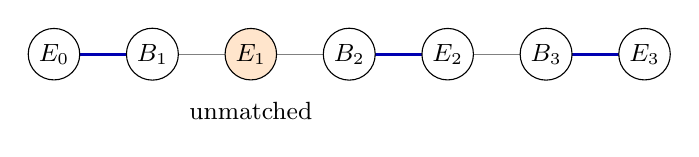
\begin{tikzpicture}[every node/.style={font=\small}]
  \draw[gray] (0,0)--(7.5,0);
  \draw[very thick,blue!70!black] (0,0)--(1.25,0);
  \draw[very thick,blue!70!black] (3.75,0)--(5,0);
  \draw[very thick,blue!70!black] (6.25,0)--(7.5,0);
  \node[draw,circle,fill=white,inner sep=2pt] at (0,0) {$E_0$};
  \node[draw,circle,fill=white,inner sep=2pt] at (1.25,0) {$B_1$};
  \node[draw,circle,fill=orange!20,inner sep=2pt] at (2.5,0) {$E_1$};
  \node[draw,circle,fill=white,inner sep=2pt] at (3.75,0) {$B_2$};
  \node[draw,circle,fill=white,inner sep=2pt] at (5,0) {$E_2$};
  \node[draw,circle,fill=white,inner sep=2pt] at (6.25,0) {$B_3$};
  \node[draw,circle,fill=white,inner sep=2pt] at (7.5,0) {$E_3$};
  \node[below=14pt] at (2.5,0) {unmatched};
\end{tikzpicture}
\caption{A maximum matching of
$E_0,B_1,E_1,B_2,E_2,B_3,E_3$ with $E_1$ left unmatched.
Blue edges are the selected adjacent pairs. In the reduction, the
unmatched even-position cloud selects the item's bin; the uniquely
forced pairs lie to its left and right.}
\label{fig:odd-path-matching}
\end{figure}

The item paths only organize the supplied membership queries. The
reduction uses singleton and adjacent-pair tests directly; no
underlying edge-query search tree is part of the instance.

\subsection{Maximum depth: bin loads become branch-height counts}

\begin{theorem}[Strong NP-completeness of maximum depth]
\label{thm:strong-worst}\label{thm:strong-height}
Deciding whether $\OPT_W(\HH)\le K$ is strongly NP-complete,
even for integer-coordinate points on a parabola, polynomially bounded
integer line coefficients, and $O(n)$ supplied binary line queries.
\end{theorem}

\begin{proofstrategy}
\begin{enumerate}
\item Force the distinguished anchor's path to attain its minimum
length. Its first-hit pairs must then be a maximum matching, with
one even-position cloud unmatched in each item path.
\item Use local cloud heights and a sorted exit histogram to exclude
internal unmatched positions. Each remaining boundary is one bin choice.
\item Moving that boundary transfers the item's size between disjoint
histogram windows. The height threshold requires every bin load to be
at most $B$, hence exactly $B$.
\end{enumerate}
\end{proofstrategy}

\subsubsection{Construction and supporting propositions}

Use the restricted 3-Partition instance of Definition~\ref{def:three-partition}.
Let $q=(p-1)(4s+2m)$ be the total matching size and $T=s-B$ the
width of a bin window. Choose a cloud offset $M$, bin levels
$\lambda_1,\ldots,\lambda_p$, and high cloud sizes $H,C$ by the
calibration in Section~\ref{sec:height-hardness-calibration}; the
decision threshold is $K=q+M$.
The source information is $a_i,B,p$; these additional quantities only
separate branch-height levels and make the distinguished path tight.

For item $i$, construct an odd path whose vertices represent clouds.
Starting with an even-position cloud of size $2$, append $p-1$
segments, indexed by $b=1,\ldots,p-1$. Each row below appends an
odd-position cloud and then the next even-position cloud.
Segment $b$ consists of one entry row, $a_i$ repetitions of the
four block rows, and one exit row:
\[
 \begin{array}{c|c|c}
 \text{part}&\text{odd-position size}&\text{next even size}\\ \hline
 \text{entry}&C&M\\
 \text{block step 1}&\lambda_b&H\\
 \text{block step 2}&\lambda_b+T&M\\
 \text{block step 3}&\lambda_{b+1}+T&H\\
 \text{block step 4}&\lambda_{b+1}&M\\
 \text{exit}&C&2
 \end{array}
\]
The repeated block is the only part depending on $a_i$.
It transfers $a_i$ units between neighboring histogram windows.
There are $4a_i+2$ odd-position vertices per segment, so the
whole item path has $2s_i+1$ vertices, where
$s_i=(p-1)(4a_i+2)$, and its maximum matching has size $s_i$.
Its $p$ even-position clouds of size $2$ are the segment boundaries.

Add one auxiliary cloud of size $M$ and cloud $0$ of size $2$.
Supply each nonzero cloud's whole-cloud singleton test, each
adjacent-pair test within an item path, and each nonanchor point's
private singleton test. Realize them by \eqref{eq:cloud-interval}
and \eqref{eq:private-singleton}.


For boundary choices, let $L_b$ be the total item size assigned to bin
$b$. Put
\[
 Q_{\mathrm{hi}}=2(p-1)(s+m),\qquad
 \beta_1=q-s,\qquad
 \beta_b=Q_{\mathrm{hi}}+2s(p-b)\quad(2\le b\le p).
\]
Here $Q_{\mathrm{hi}}$ counts the always-high pairs, and $\beta_b$
is the reference tail count in bin window $b$ after its bin load is
removed. These counts are combinatorial; their levels are calibrated later.

Soundness starts with an arbitrary adaptive tree. A tight lower
bound on the distinguished path forces its cloud groups to form
maximum matchings; only then can their heights be sorted and counted.

\begin{proposition}[Tight-spine matching normalization]
\label{prop:height-normalization}
Every identifying tree has height at least $K$. A tree of height at
most $K$ can be normalized without increasing height so its first-hit
pairs form a maximum matching in every item path, all clouds are
intact at their first hit, and the distinguished cloud's private query
is last. If $N(t)$ counts exits of local height at least $t$, sorting
those exits by nonincreasing height gives the exact criterion
\begin{equation}\label{eq:height-profile}
 t+N(t)\le K
\end{equation}
at every exit-height level.
\end{proposition}

The odd-path lemma allows every even position to be unmatched,
but only the designated boundaries should represent bins. One height
level detects and excludes all internal positions at once.

\begin{proposition}[Only boundary positions are feasible]
\label{prop:height-boundaries}
Every matching whose normalized tree fits height $K$ leaves a
boundary cloud unmatched in each item path. Its $p$ possible boundaries choose the item's bin.
\end{proposition}

With internal positions excluded, moving an unmatched boundary is
a genuine bin choice. Its effect on the exit histogram adds across
items, turning the height constraints into bin-capacity constraints.

\begin{proposition}[Histogram windows encode bin loads]
\label{prop:height-windows}
At the upper level $t_b=\lambda_b+T$ of each bin window,
\[
 N(t_b)=\beta_b+L_b,\qquad t_b+\beta_b=K-B.
\]
Consequently the height criterion requires $L_b\le B$ for every bin.
\end{proposition}

The bin windows establish the necessary conditions. For the reverse
direction, balanced loads must also respect every remaining height
level and identify all cloud points, including the distinguished cloud.

\begin{proposition}[Balanced loads give a complete tree]
\label{prop:height-completeness}
Boundary matchings with $L_b=B$ satisfy every height-profile constraint
and yield a complete identifying tree of height $K$.
\end{proposition}

The combinatorial equivalence must be accompanied by a size bound.
Explicit clouds and integer lines preserve strong hardness only if
their replication and numerical values stay polynomial.

\begin{proposition}[Polynomial geometric encoding]
\label{prop:height-encoding}
The construction has polynomial size on the restricted source input,
integer coordinates and coefficients bounded by $O(n^4)$, and $O(n)$
supplied strict binary lines. A height-$K$ identifying tree is a
polynomially checkable NP certificate.
\end{proposition}

\begin{proof}[Proof of Theorem~\ref{thm:strong-worst}]
A source partition yields a height-$K$ tree by
Proposition~\ref{prop:height-completeness}. Conversely, normalize any
height-$K$ tree by Proposition~\ref{prop:height-normalization};
Propositions~\ref{prop:height-boundaries} and~\ref{prop:height-windows}
give bin loads at most $B$. Since their sum is $s=pB$ across $p$ bins,
every load must equal $B$. Each such bin contains three items: two
items sum to less than $B$, while four sum to more than $B$, by the
source promise $B/4<a_i<B/2$. These groups form a 3-partition.
Proposition~\ref{prop:height-encoding} supplies strong polynomial
encoding and NP membership. Thus the reduction is exact for arbitrary
adaptive trees.
\end{proof}

\subsubsection{Technical proofs of the height propositions}

\begin{proof}[Proof of Proposition~\ref{prop:height-normalization}]
We normalize in two stages. First, counting the queries unavoidable
on the distinguished anchor's path forces maximum matchings and intact
cloud exits. Then sorting those exits gives the complete height test.

\begin{claim}[The distinguished anchor forces maximum matchings]
\label{clm:height-tight-anchor}
Every identifying tree has height at least $K$. If its height is at
most $K$, the first-covered pairs form a maximum matching in every
item path, and no nonzero-cloud private test is asked on the anchor
path.
\end{claim}
\begin{proof}
Follow the anchor of cloud $0$ through any complete tree. It needs the private
test for the other point of cloud $0$. Private tests of other
clouds do not distinguish their anchors from this anchor.
It therefore also needs cloud queries covering the $2q+m$ item-path
anchors and the auxiliary anchor.

Classify each anchor by its first hitting cloud query along this
all-miss path. A query first covers one anchor or two adjacent
anchors. The first-covered pairs are disjoint, hence form a
matching of size at most $\sum_i s_i=q$.
There are $2q+m+1$ nonzero anchors to cover. If $g$ first-covered
groups are pairs, the remaining groups are singletons, so the path
uses $(2q+m+1)-g$ cloud queries. Since $g\le q$, this is at least
$q+m+1$. It must also ask the private query separating the two
points of cloud $0$, giving the lower bound
$q+m+2=K$, where the equality uses $M=m+2$ and $K=q+M$
from Section~\ref{sec:height-hardness-calibration}.

If a tree has height at most $K$, equality holds. No private test
of a nonzero cloud can occur on this path, and its pairs form a
maximum matching in every item path. Lemma~\ref{lem:odd-path}
therefore leaves exactly one even-position cloud unmatched per item.
\end{proof}

Claim~\ref{clm:height-tight-anchor} gives equality on the
distinguished path. Before a cloud's first whole-cloud query, each of
its points answers every earlier whole-cloud query just as its anchor
does. The only supplied queries that can separate a nonanchor from
its anchor are private tests, and Claim~\ref{clm:height-tight-anchor}
excludes those from this path. Thus each first-hit exit contains one
whole cloud or, for a pair query, two whole clouds.
Replace any query first covering just one cloud by its supplied
whole-cloud singleton test. Put cloud $0$'s private query last;
this advances the other exits and leaves its two points within
depth $K$. Attach the optimal local codes of
Lemma~\ref{lem:cloud-heights}.

After normalization, each exit has an independent local height.
Its only interaction with the other exits is its spine position,
so sorting reduces all depth constraints to one tail-count criterion.

\begin{claim}[Sorting exit heights gives the complete depth test]
\label{clm:height-sorted-profile}
After the cloud-query groups are sorted by nonincreasing local
height, every target path has depth at most $K$ exactly when
$t+N(t)\le K$ at every exit-height level $t$.
\end{claim}
\begin{proof}
The cloud queries now act on disjoint singletons and pairs.
By Lemma~\ref{lem:cloud-heights}, their exit heights are $w-1$
for a singleton and $\max\{u,v\}$
for a pair. Include the final private query as an exit of height
zero. For consecutive heights $r<s$, the old maximum is
$\max\{j+r,j+1+s\}=j+1+s$. After exchanging them,
both $j+s$ and $j+1+r$ are at most $j+1+s$, so the new maximum
cannot be larger. Adjacent exchanges therefore sort the heights
nonincreasingly without increasing any overall height bound.

Write $h_j$ for the local height of the exit at spine position $j$.
The \emph{tail histogram} of exit heights is
$N(t)=|\{j:h_j\ge t\}|$, the number of exits of height at least $t$.
In sorted order, for every realized exit-height level $t$,
the last exit counted by $N(t)$ has height exactly $t$ and position
$N(t)$. Thus $t+N(t)$ is an actual route depth. Conversely, for
any exit at position $j$, $j\le N(h_j)$, so
$j+h_j\le N(h_j)+h_j$. These two inequalities prove
\[
 \max_j(j+h_j)=\max_{t\text{ an exit height}}(t+N(t)).
\] Thus all target paths fit within $K$ exactly when
\eqref{eq:height-profile} holds at every exit-height level $t$.
Thus the depth test reduces to the largest sum of spine position and
remaining local depth over all exits.
\end{proof}
\end{proof}

\begin{proof}[Proof of Proposition~\ref{prop:height-boundaries}]
Every matched pair has exit height at least $M$, because each odd
cloud has size at least $\lambda_1=M$. The auxiliary singleton has exit
height $M-1$. An unmatched internal even vertex has size $M$ or $H$,
and hence exit height at least $M-1$.
At $t=M-1$, these give
$N(t)\ge q+1+\text{number of such internal unmatched vertices}$.
If there are $c$ internal unmatched vertices, then
$(M-1)+N(M-1)\ge(M-1)+(q+1+c)=K+c$.
Claim~\ref{clm:height-sorted-profile} permits at most $K$ at this
level, so $c=0$.
The unmatched vertex in each item path therefore chooses one of
its $p$ boundary positions, interpreted as a bin.
\end{proof}

\begin{proof}[Proof of Proposition~\ref{prop:height-windows}]
To read bin loads from the histogram, first compute the effect
of crossing one segment. These local transfers telescope across
segments; a reference matching then fixes the baseline counts.

\begin{claim}[A segment transfers load only between its neighboring windows]
\label{clm:height-segment-transfer}
Its two boundary matchings differ by the window transfer of item $i$.
\end{claim}
\begin{proof}
By Lemma~\ref{lem:odd-path}, moving the unmatched vertex across
segment $b$ reverses all its left/right pairing choices. Applying
Lemma~\ref{lem:cloud-heights} to those two matchings gives their
exit heights as follows.
When its unmatched vertex is before the segment, a repeated block
has heights
\[
 H,\ \lambda_b+T,\ H,\ \lambda_{b+1}.
\]
When that vertex is after the segment, the same block has heights
\[
 \lambda_b,\ H,\ \lambda_{b+1}+T,\ H.
\]
The two connector pairs have height $C$ in either case.
With $a_i$ repetitions, the change in $N(t)$ is exactly
\[
 -a_i\mathbf1_{(\lambda_b,\lambda_b+T]}(t)+
  a_i\mathbf1_{(\lambda_{b+1},\lambda_{b+1}+T]}(t).
\]
The windows are disjoint because $T<s$ and consecutive
$\lambda_b$ differ by at least $s$. Write
$W_j=(\lambda_j,\lambda_j+T]$. Moving from boundary 1 to
boundary $b$ adds the changes of segments $1,\ldots,b-1$:
\[
 a_i\sum_{j=1}^{b-1}
       (-\mathbf1_{W_j}+\mathbf1_{W_{j+1}})
 =-a_i\mathbf1_{W_1}+a_i\mathbf1_{W_b}.
\]
Each intermediate window occurs once with each sign and cancels.
For $b=1$ the sum is empty and the displayed difference is zero.
Thus the item removes $a_i$ from window 1 and adds it to its chosen
window $b$. Figure~\ref{fig:hardness-window-transfer}
illustrates this change relative to the reference matching.
\end{proof}
The transfer calculation gives each item's change in the tail count.
Taking the all-first-bin matching as a reference and summing these
changes yields the tail count needed by the height criterion.

\begin{claim}[Reference tail counts turn transfers into bin loads]
\label{clm:height-bin-counts}
At $t_b=\lambda_b+T$, the resulting count is $N(t_b)=\beta_b+L_b$.
\end{claim}
\begin{proof}
In the reference matching assigning all items to bin 1,
$Q_{\mathrm{hi}}$ pairs have height $H$ or $C$.
For each segment $c=1,\ldots,p-1$, the remaining pairs comprise
$s$ of height $\lambda_c+T$ and $s$ of height $\lambda_{c+1}$.
Consider a threshold $t$ in window $b$, so
$\lambda_b<t\le\lambda_b+T$. If $c<b$, then both heights in
segment $c$ are below $t$: in particular,
$\lambda_{c+1}\le\lambda_b<t$. If $c\ge b$, both heights are
at least $t$, since $\lambda_c+T\ge\lambda_b+T\ge t$ and
$\lambda_{c+1}>\lambda_b+T$. Thus, for $b\ge2$, precisely the
$p-b$ segments $c=b,\ldots,p-1$ contribute their two batches of
$s$ pairs, giving the reference count
$Q_{\mathrm{hi}}+2s(p-b)=\beta_b$. In the first window all
$p-1$ segments contribute, so the count is
$Q_{\mathrm{hi}}+2s(p-1)=q=\beta_1+s$.
Summing Claim~\ref{clm:height-segment-transfer} over items changes the first reference count
by $-(s-L_1)$ and changes each later reference count by $L_b$.
Thus throughout each window, and at its upper level,
$N(t_b)=\beta_b+L_b$. For the offset identity, first use
$\lambda_1=M$, $T=s-B$, and $\beta_1=q-s$ to get
\[
 t_1+\beta_1=M+(s-B)+(q-s)=K-B.
\]
For $b\ge2$, substitute the calibrated levels and reference counts:
\begin{align*}
 t_b+\beta_b
 &=M+(2b-3)s+(s-B)+Q_{\mathrm{hi}}+2s(p-b)\\
 &=M-B+Q_{\mathrm{hi}}+2s(p-1)\\
 &=M-B+2(p-1)(s+m)+2s(p-1)=K-B.
\end{align*}
The second line collects the $s$ terms, whose coefficient is
$(2b-3)+1+2(p-b)=2(p-1)$. The third substitutes
$Q_{\mathrm{hi}}=2(p-1)(s+m)$; the last equality uses
$q=(p-1)(4s+2m)$ and $K=M+q$.
The profile condition at this level is
$t_b+N(t_b)\le K$, or equivalently $L_b\le B$.
Thus \eqref{eq:height-profile} requires $L_b\le B$ for every bin.
Since $\sum_b L_b=s=pB$, all these inequalities are equalities
and yield a source 3-partition.
\end{proof}
\end{proof}

\begin{proofstrategy}
List every possible exit height and compute its tail count for balanced
loads. The table checks the profile at each such level; between levels
the tail count is constant, so the profile expression can only increase
up to the next listed height. Sorting the exits and attaching their
local codes then constructs the required tree.
\end{proofstrategy}
\begin{proof}[Proof of Proposition~\ref{prop:height-completeness}]
Choose the boundary matchings of a source partition, so $L_b=B$.
Proposition~\ref{prop:height-windows} shows that the window upper
levels satisfy \eqref{eq:height-profile} with equality.
For completeness, the remaining levels have the following counts.
Lemma~\ref{lem:cloud-heights} and the construction table enumerate
the possible local heights. Cloud $0$'s final private exit has height
$0$, each unmatched boundary cloud has size $2$ and singleton height
$1$, and the auxiliary cloud of size $M$ has singleton height $M-1$.
The repeated-block pairs have heights among
$H,\lambda_b,\lambda_b+T,\lambda_{b+1},\lambda_{b+1}+T$,
while the connector pairs have height $C$. Hence the only possible
levels are $0,1,M-1,H,C,\lambda_b,$ and $\lambda_b+T$; the last
levels $\lambda_b+T$ were already checked by
Proposition~\ref{prop:height-windows}.
\[
 \begin{array}{c|c|c}
 t&N(t)&t+N(t)\\ \hline
 0&K&K\\
 1&K-1&K\\
 M-1&q+1&K\\
 \lambda_b&\beta_b+s&K\\
 H&Q_{\mathrm{hi}}&K\\
 C&2m(p-1)&K-2s(p-1)+1\le K
 \end{array}
\]
To verify the table, there are $q+m+1=K-1$ nonzero cloud groups
and the final height-zero private exit. This gives the first two rows.
At $M-1$, precisely the $q$ pairs and the auxiliary cloud count;
unmatched boundary clouds have height one. At $\lambda_b$, the
transfer windows exclude their lower endpoint, so the count is its
reference value $\beta_b+s$. For $b=1$ this gives
$\lambda_1+\beta_1+s=M+q=K$; for $b\ge2$ it gives
\[
 \lambda_b+\beta_b+s
 =M+Q_{\mathrm{hi}}+2s(p-1)=M+q=K.
\]
There are two height-$H$ pairs per repeated block and two height-$C$
connectors per segment, totaling $Q_{\mathrm{hi}}$. Hence
$H+Q_{\mathrm{hi}}=M+q=K$, whereas
\[
 C+2m(p-1)=K-2s(p-1)+1\le K
\]
because $p\ge2$ and $s\ge1$. These are all possible exit heights,
together with the already checked $\lambda_b+T$. The count $N(t)$ is constant between
successive exit heights, so $t+N(t)$ increases there and its maximum
occurs at a listed exit height. Sort the corresponding queries, attach
their exact one- or two-cloud codes, and finish with cloud $0$'s
private query. This constructs a complete tree of height $K$.
\end{proof}

\begin{proofstrategy}
Bound the number and size of clouds first, then use those bounds to
control point coordinates and line coefficients. Count the supplied
queries separately, and finish by bounding the size and verification
time of a proper identifying-tree certificate.
\end{proofstrategy}
\begin{proof}[Proof of Proposition~\ref{prop:height-encoding}]
There are $2q+m+2$ clouds, each of size at most
$C=O(ps+m)$. Their total number of hypotheses is polynomial in
the restricted source input. For the explicit geometric bounds, each
cloud size and its index are at most the total point count $n$,
and $Q=4\max_iw_i\le4n$. Thus every abscissa satisfies
$0\le Qi+j\le4n^2+n=O(n^2)$, and every ordinate is $O(n^4)$.
The cloud-query coefficient $4Q(a+b)$ is $O(n^2)$ and its
constant $Q^2(2a-1)(2b+1)$ is $O(n^4)$. The private-query
coefficients $4t$ and $2t^2-1$ have the same bounds. There is
one private query per nonanchor and at most twice the number of
clouds in singleton and path-edge queries, so there are $O(n)$
supplied lines. Every proper identifying tree has $n-1$ internal nodes;
its answers and height can be checked in polynomial time.
This proves membership in NP and strong NP-hardness with
polynomially bounded numerical data.
\end{proof}

\subsubsection{Calibration of the height construction}
\label{sec:height-hardness-calibration}

\begin{parameterchoice}
Choose
\[
 \begin{aligned}
 M&=m+2,&\lambda_1&=M,\\
 \lambda_b&=M+(2b-3)s\quad(2\le b\le p),&
 H&=M+2s(p-1),\qquad C=H+1.
 \end{aligned}
\]
The width $T=s-B<s$ makes the windows disjoint. All block levels are
below $H$, and the connectors have height $C$. These choices give
$t_b+\beta_b=K-B$ and make the minimum distinguished-path length
$q+m+2$ exactly $K=q+M$.
\end{parameterchoice}

\begin{figure}[tbp]
\centering
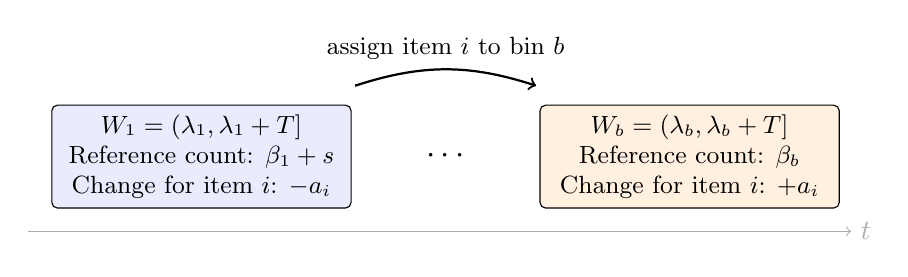
\begin{tikzpicture}[
  window/.style={draw,rounded corners=2pt,minimum width=3.8cm,
                 minimum height=1.15cm,align=center,font=\small}
]
  \node[window,fill=blue!8] (windowone) at (0,0)
    {$W_1=(\lambda_1,\lambda_1+T]$\\
     Reference count: $\beta_1+s$\\
     Change for item $i$: $-a_i$};
  \node[font=\large] at (3.1,0) {$\cdots$};
  \node[window,fill=orange!12] (windowb) at (6.2,0)
    {$W_b=(\lambda_b,\lambda_b+T]$\\
     Reference count: $\beta_b$\\
     Change for item $i$: $+a_i$};
  \draw[->,thick] (1.95,0.9) to[bend left=18]
    node[above,font=\small] {assign item $i$ to bin $b$}
    (4.25,0.9);
  \draw[->,gray!65] (-2.2,-0.95)--(8.25,-0.95)
    node[right] {$t$};
\end{tikzpicture}
\caption{Relative to the reference matching, assigning one item of
size $a_i$ from bin 1 to bin $b$ removes $a_i$ from the first
histogram window and adds $a_i$ to window $b$; intermediate windows
are unchanged. Superposing the item transfers gives
$N(t)=\beta_j+L_j$ throughout window
$W_j=(\lambda_j,\lambda_j+T]$.}
\label{fig:hardness-window-transfer}
\end{figure}

\subsection{Expected depth: an exact matching formula}

The expected-depth reduction needs no clouds. Each nonzero
hypothesis is one path vertex or one isolated vertex, and every
query isolates either a singleton or an adjacent pair.
The combinatorial choice is still a matching, but its objective
depends on how the resulting pairs are ordered.

For a finite positive weight vector $z$, keeping repeated values
as distinct entries, define the \emph{weighted completion sum} by
\[
 \mathcal C(z)=\sum_{j=1}^{|z|}jz_{(j)},
 \qquad z_{(1)}\ge\cdots\ge z_{(|z|)}.
\]
It equals the sum of the individual weights plus the smaller
weight for each unordered pair of entries: in decreasing order,
an earlier entry delays a later entry by one. Thus concatenating
vectors $u,v$ adds the cross contribution
$\sum_{i,j}\min\{u_i,v_j\}$.
Equivalently,
if $h_z(t)=|\{j:z_j\ge t\}|$, then
\begin{equation}\label{eq:completion-histogram}
 \mathcal C(z)=\int_0^\infty
                 \frac{h_z(t)(h_z(t)+1)}2\,dt.
\end{equation}
At height $t$, the first $h_z(t)$ ranks contribute
$1+\cdots+h_z(t)$; integrating those contributions proves the identity.

The completion sum becomes a tree objective once first-hit groups
are identified with a matching. This correspondence must hold for
arbitrary adaptive trees as well as for the sorted constructions.

\begin{lemma}[Exact singleton/pair formula]\label{lem:pair-invoice}
Consider a \emph{linear forest}, meaning a disjoint union of paths
(isolated vertices are allowed), with vertices $1,\ldots,N$ ordered
component by component. Represent them and a distinguished hypothesis by
$(i,i^2)$, $0\le i\le N$. Supply $I_{i,i}$ for each nonzero vertex
and $I_{i,i+1}$ for each forest edge.
Give the distinguished hypothesis weight $\omega_0>0$ and the
others positive weights $\omega_v$.
For a matching $\mathcal M$, let $J(\mathcal M)$ be the vector
containing mass
$\omega_u+\omega_v$ for each matched pair and $\omega_v$ for each
unmatched vertex, retaining multiplicities when masses coincide.
The optimal unnormalized expected depth is
\begin{equation}\label{eq:pair-invoice}
 \min_{\mathcal M}
 \left\{\omega_0(N-|\mathcal M|)
       +\mathcal C(J(\mathcal M))
       +\sum_{\{u,v\}\in\mathcal M}(\omega_u+\omega_v)\right\}.
\end{equation}
If $\omega_0>N\sum_{v>0}\omega_v$, an optimal matching in this
formula has maximum cardinality.
\end{lemma}
\begin{proofstrategy}
Read any tree from the distinguished all-miss spine: its disjoint
first-hit pairs form a matching. Then sort the group masses; adjacent
exchanges minimize first-cover cost. A sufficiently heavy distinguished
point forces maximum cardinality before any other cost matters.
\end{proofstrategy}
\begin{proof}
We first establish the invoice in both directions: extract its
terms from any adaptive tree, and realize them for any matching.
The distinguished-weight condition is a separate restriction applied
afterward.

\begin{claim}[First-hit groups attain the matching cost]
\label{clm:pair-invoice-attainable}
The spine contributes one query per singleton or matched pair, and
only a pair requires an extra local query.
\end{claim}
\begin{proof}
Follow hypothesis $0$, which misses every supplied membership query.
The hypotheses first covered together are disjoint singletons
or adjacent pairs. The pairs form a matching $\mathcal M$,
and the spine has $N-|\mathcal M|$ queries.
A pair's hit branch requires exactly one additional query;
a singleton branch requires none.
This gives the first and third terms of \eqref{eq:pair-invoice}.

For the first-cover term, suppose masses $a<b$ occupy consecutive
positions $j,j+1$. Their contribution is
$ja+(j+1)b$ in that order and $jb+(j+1)a$ after swapping, a decrease
of $b-a$. Repeated exchanges show that nonincreasing mass is optimal.
Every such ordering is executable: query the selected pairs
and the singleton tests for the unmatched vertices in that order.
The groups are disjoint, so each query's hit branch exits only
to its own group. This proves the
formula both as a lower bound on arbitrary trees and as an
attainable value for each matching.
\end{proof}

The exact invoice still permits matchings of different sizes. Giving
the distinguished point enough weight makes its spine length decisive,
so later gadget calculations need consider only maximum matchings.

\begin{claim}[The distinguished weight forces maximum cardinality]
\label{clm:pair-invoice-cardinality}
Under the stated dominance condition, minimizing its depth is the
first objective.
\end{claim}
\begin{proof}

Every proper complete tree has depth at most $N$, so the total
weighted depth of all nonzero hypotheses is at most
$N\sum_{v>0}\omega_v$. One additional query on hypothesis $0$'s
path outweighs this entire budget under the stated inequality.
An optimal tree must consequently minimize that path's length,
which means choosing a maximum-cardinality matching.
\end{proof}
\end{proof}

\subsection{Expected depth: bin loads become a quadratic penalty}

\begin{theorem}[Strong NP-completeness of expected depth]
\label{thm:strong-average}
Given supplied binary lines, strictly positive integer hypothesis
weights bounded by a fixed polynomial in $n$, and a rational threshold,
deciding the optimal expected depth is strongly NP-complete.
This holds for $\HH=\{(i,i^2):0\le i<n\}$, $O(n)$ integer-coefficient
lines, and negative answer classes of size at most two.
\end{theorem}

\begin{proofstrategy}
\begin{enumerate}
\item Use the exact matching cost formula and a heavy distinguished point
to normalize the optimum to one unmatched even vertex per item.
\item Pair-mass histograms encode bin loads. Integrating their tail
counts produces a quadratic load penalty and an unwanted linear term.
\item Tiny, ordered boundary-weight adjustments cancel that linear
term. Medium-weight isolated vertices exclude internal choices, and
scale separation makes rounding smaller than a unit imbalance.
\end{enumerate}
\end{proofstrategy}

\subsubsection{Construction and supporting propositions}

Let $q=2s(p-1)$ be the total matching size and define the reference
bin counts
\[
 \beta_1=q-s,\qquad \beta_b=2s(p-b)\quad(2\le b\le p).
\]
Take an isolated-vertex count $r$, an even window width $V$, and bin
levels $\lambda_b$ from Section~\ref{sec:average-hardness-calibration}.
The $r$ isolated vertices have weight $Z=V/2$. To cancel the bin
linear term, define
\[
 \begin{aligned}
 t_i&=q+r+m-i,&
 \delta_{ib}&=\left\lfloor\frac{V(\beta_1-\beta_b)a_i}{t_i}\right\rfloor,\\
 D&=\max_{i,b}\delta_{ib},& A_i&=1+(2D+1)i.
 \end{aligned}
\]
Here $t_i$ will be the exact coefficient of unmatched item $i$;
$A_i$ fixes the unmatched-weight order, and $\delta_{ib}$ is its small
bin-dependent correction. Since
$\beta_1-\beta_b=(2b-3)s>0$ for $b\ge2$, all corrections are
nonnegative and $\delta_{i1}=0$.

For item $i$, form an odd path
\[
 E_{i0},\,B_{i1},\,E_{i1},\,\ldots,\,
 B_{is_i},\,E_{is_i},\qquad s_i=2a_i(p-1),
\]
where each displayed symbol also denotes that vertex's weight.
First define unperturbed even weights
\[
 E^0_{ij}=
 \begin{cases}
 A_i,&j\equiv0\pmod{2a_i},\\
 A_i+V,&j\text{ odd},\\
 A_i+2V,&\text{otherwise}.
 \end{cases}
\]
Each consecutive difference is $+V$ or $-V$.
Between two boundary positions there are $2a_i$ steps,
of which $a_i$ go up and $a_i$ go down.
For $1\le j\le s_i$ let $b=\lceil j/(2a_i)\rceil$ and put
\[
 B_{ij}=
 \begin{cases}
 \lambda_b-E^0_{i,j-1},&E^0_{ij}-E^0_{i,j-1}=V,\\
 \lambda_{b+1}-E^0_{ij},&E^0_{ij}-E^0_{i,j-1}=-V.
 \end{cases}
\]
Finally set
$E_{i,2a_i(b-1)}=A_i+\delta_{ib}$ at each of the $p$ boundaries
and leave all other even weights unperturbed.
The odd weights do not change when this adjustment is made.

Add $r$ isolated forest vertices of weight $Z$.
The nonzero forest has $N=2q+m+r$ vertices, with maximum matching
size $q$. Let $P$ be the total weight of its item-path vertices,
$W=P+rZ$, and give hypothesis $0$ weight
$\omega_0=(N+1)W+1$.
Use precisely the lines of Lemma~\ref{lem:pair-invoice}.
Normalize the weights only after the construction.


Use $E_+=q\sum_{i,b}\delta_{ib}$ for the possible pair-mass
perturbation and $E_-=\sum_i(t_i-1)$ for the rounding loss.
Write $G$ for the minimum raw weighted cost for a fixed maximum
matching in Lemma~\ref{lem:pair-invoice}, $U=(U_1,\ldots,U_m)$ for
its unmatched item weights, and $z$ for its $q$ pair masses. Boundary choice $b_i$
assigns item $i$ to that bin, whose load is
$L_b=\sum_{i:b_i=b}a_i$.

The three weight classes serve different purposes: pair masses
carry the histogram, isolated vertices penalize internal choices, and
small boundary weights permit controlled corrections. Their separation
also fixes the orders used in the invoice.

\begin{proposition}[Separated scales and maximum-matching normalization]
\label{prop:average-normalization}
All weights are positive. Every pair mass exceeds $Z$ and every
unmatched item weight; boundary weights are below $Z$ and ordered by
item index. The optimum uses a maximum-cardinality matching, and the
calibration ensures $E_++E_-<V$.
\end{proposition}

Once matching cardinality is fixed, the distinguished contribution
and several cross terms are constant. The remaining completion and
unmatched-vertex costs vary with the bin choices, so we record their
sum in the matching cost formula below.

\begin{proposition}[The matching-dependent invoice]
\label{prop:average-invoice}
\begin{equation}\label{eq:expected-remaining-invoice}
 G=G_{\mathrm{fix}}+\mathcal C(z)+\mathcal C(U)
       +(q-1)\sum_i U_i+r\sum_i\min\{U_i,Z\},
\end{equation}
where
\[
 G_{\mathrm{fix}}=
 \omega_0(q+m+r)+\frac{Zr(r+1)}2+qrZ+P.
\]
\end{proposition}

For boundary matchings, the same transfer idea now changes pair
masses. The completion integral converts their tail counts into a
quadratic load term and a linear term.

\begin{proposition}[Pair windows give a quadratic load identity]
\label{prop:average-windows}
Let $b_i$ be the bin chosen by item $i$ and
$L_b=\sum_{i:b_i=b}a_i$. Let $z^0$ be the unperturbed pair-mass
vector for these choices, and let $C_{\mathrm{ref}}$ be the
completion sum of the reference vector in which every item chooses
bin $1$. Then
\begin{equation}\label{eq:expected-bin-identity}
 \mathcal C(z^0)=C_{\mathrm{ref}}+
 V\left[\sum_b\beta_bL_b-\beta_1s+
             \frac{\sum_bL_b^2-s^2}{2}\right].
\end{equation}
\end{proposition}

A quadratic penalty favors balanced loads only after the bin-dependent
linear term is removed. The boundary corrections perform that
cancellation, and the error bounds preserve a strict threshold gap.

\begin{proposition}[Boundary corrections cancel the linear term]
\label{prop:average-boundary-gap}
For every boundary matching, there is an error $e$ with
$-E_-\le e\le E_+$ such that
\begin{equation}\label{eq:expected-quadratic-gap}
 G=G_{\mathrm{fix}}+\sum_i t_iA_i+C_{\mathrm{ref}}+
       \frac V2\left(\sum_bL_b^2-s^2\right)+e.
\end{equation}
Define the raw threshold
\begin{equation}\label{eq:expected-raw-threshold}
 k_0=G_{\mathrm{fix}}+\sum_i t_iA_i+C_{\mathrm{ref}}
              +\frac V2(pB^2-s^2),\qquad k=k_0+E_+.
\end{equation}
A boundary matching has $G\le k$ exactly when every bin load is $B$.
\end{proposition}

The quadratic calculation concerns boundary choices. Full soundness
also requires excluding internal unmatched vertices; the isolated
vertices provide that penalty without introducing nonpolynomial data.

\begin{proposition}[Internal choices are excluded; encoding is strong]
\label{prop:average-internal-encoding}
Every maximum matching with an internal unmatched even vertex has
$G>k$. The construction and its normalized threshold $k/\Omega$,
where $\Omega=\omega_0+W$, have polynomially bounded numerical data
and $O(n)$ supplied lines; a proper tree is a polynomial NP certificate.
\end{proposition}

\begin{proof}[Proof of Theorem~\ref{thm:strong-average}]
A source partition selects boundary choices of raw cost at most $k$
by Proposition~\ref{prop:average-boundary-gap}. Conversely,
Proposition~\ref{prop:average-normalization} reduces the optimum to
maximum matchings. Proposition~\ref{prop:average-internal-encoding}
excludes internal unmatched vertices, so every unmatched item position
chooses a boundary and hence a bin. Proposition~\ref{prop:average-boundary-gap}
shows that a qualifying matching has every bin load equal to $B$.
Because two source items sum to less than $B$ and four sum to more than
$B$, each such bin contains exactly three items; the chosen bins
therefore give a 3-partition. Normalizing divides both objective and
threshold by $\Omega$, while the encoding proposition supplies strong
hardness and NP membership, including arbitrary adaptive trees.
\end{proof}

\subsubsection{Technical proofs of the expected-depth propositions}

\begin{proofstrategy}
Compare the weight classes in turn: pair masses must dominate unmatched
and isolated weights, while boundary weights must stay below the
isolation threshold and retain their item order. These inequalities
activate the invoice lemma's maximum-cardinality criterion.
\end{proofstrategy}
\begin{proof}[Proof of Proposition~\ref{prop:average-normalization}]
The scale estimates verified in Section~\ref{sec:average-hardness-calibration}
are used here only to compare the three weight classes.
Every even weight is positive. By the first bound in
\eqref{eq:expected-scale-bounds}, $A_i+\delta_{ib}<V/100$, so
$A_i+2V<2.01V$ and every unmatched even weight is below $3V$.
For an upward step, the two possible pair masses are
$\lambda_b$ and $\lambda_b+V$; for a downward step they are
$\lambda_{b+1}+V$ and $\lambda_{b+1}$. Since
$\lambda_b\ge12V$ and $\lambda_{b+1}\ge14V$, all these masses are
at least $12V$. Boundary adjustments are nonnegative and can only
increase a matched pair's mass. The odd weights are also positive:
each is either $\lambda_b-E^0_{i,j-1}$ or
$\lambda_{b+1}-E^0_{ij}$, and every unperturbed even weight is
less than $2.01V$. Hence every pair mass exceeds $Z=V/2$ and every
unmatched even weight.
Boundary weights are below $Z$, and they increase strictly with the
item index: $A_{i+1}-(A_i+D)=D+1>0$. Finally,
$E_++E_-<V$ follows from the last two calibration bounds.
Here $\omega_0=(N+1)W+1>NW$, so the dominance condition of
Lemma~\ref{lem:pair-invoice} restricts the optimum to maximum
matchings. By Lemma~\ref{lem:odd-path}, each item then leaves
one even vertex unmatched.
\end{proof}

\begin{proof}[Proof of Proposition~\ref{prop:average-invoice}]
Split the completion sum into $z,U$, and the vector of $r$
isolated weights $Z$. Its within-vector terms are
$\mathcal C(z)$, $\mathcal C(U)$, and $Zr(r+1)/2$.
Proposition~\ref{prop:average-normalization} puts every pair mass
above every unmatched and isolated weight. Thus the minimum-weight
cross-term identity preceding \eqref{eq:completion-histogram} gives
cross terms
$q\sum_iU_i$ and $qrZ$. The unmatched/isolated cross term is
$r\sum_i\min\{U_i,Z\}$. Thus the total completion term is
\[
 \mathcal C(z)+\mathcal C(U)+\frac{Zr(r+1)}2
       +q\sum_iU_i+qrZ+r\sum_i\min\{U_i,Z\}.
\]
The item paths partition into matched vertices and the unmatched
vertices, so the extra local pair cost is $P-\sum_iU_i$.
The witness path has $N-q=q+m+r$ queries and costs
$\omega_0(q+m+r)$. Adding these terms replaces $q\sum_iU_i$
by $(q-1)\sum_iU_i$ and gives the displayed
$G_{\mathrm{fix}}$, proving the invoice.
\end{proof}

\begin{proof}[Proof of Proposition~\ref{prop:average-windows}]
We first determine the pair-mass histogram for each boundary choice,
then integrate it. This separates the local matching calculation
from the algebra that produces the quadratic objective.

\begin{claim}[Boundary movement transfers pair masses between windows]
\label{clm:average-mass-transfer}
The pair-mass tail count in window $b$ is $\beta_b+L_b$, and it is unchanged outside the windows.
\end{claim}
\begin{proof}
By Lemma~\ref{lem:odd-path}, unmatching boundary $2a_i(b-1)$
fixes all left and right pairs and assigns item $i$ to bin $b$.
Temporarily omit the boundary perturbations and denote the
resulting pair-mass vector by $z^0$.
For an upward step in segment $b$, pairing its odd vertex
to the even vertex on the left gives mass $\lambda_b$,
while pairing right gives $\lambda_b+V$.
For a downward step, those masses are
$\lambda_{b+1}+V$ and $\lambda_{b+1}$.
Moving the unmatched vertex across a whole segment consequently
changes the pair-mass histogram by
\[
 -a_i\mathbf1_{(\lambda_b,\lambda_b+V]}+
  a_i\mathbf1_{(\lambda_{b+1},\lambda_{b+1}+V]}.
\]
There are exactly $a_i$ steps of each type.
Write $W_j=(\lambda_j,\lambda_j+V]$. Moving an item from
boundary 1 to boundary $b_i$ adds
\[
 a_i\sum_{j=1}^{b_i-1}
       (-\mathbf1_{W_j}+\mathbf1_{W_{j+1}})
 =-a_i\mathbf1_{W_1}+a_i\mathbf1_{W_{b_i}}.
\]
For $b_i=1$ this is zero; otherwise each intermediate indicator
cancels. This is the same telescoping mechanism as in the height
construction.
In the reference matching, all odd vertices are paired to their
right. Segment $b$ contributes $s$ masses $\lambda_b+V$ and
$s$ masses $\lambda_{b+1}$ after summing over items.
For a threshold $t$ in window $b$, where
$\lambda_b<t\le\lambda_b+V$, a segment $c<b$ contributes no mass:
its larger mass is $\lambda_{c+1}\le\lambda_b<t$. Every segment
$c\ge b$ contributes both batches, since
$\lambda_c+V\ge\lambda_b+V\ge t$ and
$\lambda_{c+1}>\lambda_b+V$. Therefore, when $b\ge2$, the
$p-b$ segments $c=b,\ldots,p-1$ contribute $2s(p-b)=\beta_b$
masses in total. In the first window all $p-1$ segments contribute,
so the reference count is $q=2s(p-1)=\beta_1+s$.
Assigning items according to loads $L_b$
changes the tail count throughout window $b$ to
$\beta_b+L_b$: the first window loses $s-L_1$ pair masses from its
reference count $q$, while each later window gains $L_b$.
Outside these disjoint windows the tail histogram is unchanged.
\end{proof}
The histogram now depends on the matching only through bin loads.
Integrating the triangular count polynomial reveals both the desired
imbalance penalty and the linear term that the next proposition
must cancel.

\begin{claim}[Integrating the tail counts yields the quadratic term]
\label{clm:average-integrated-windows}
The triangular histogram formula gives \eqref{eq:expected-bin-identity}.
\end{claim}
\begin{proof}
Let $C_{\mathrm{ref}}$ be the completion sum of the unperturbed
pair masses when every first boundary is unmatched. It is explicitly
computable by sorting those $q$ masses.
Let $f(h)=h(h+1)/2$. Direct expansion gives
\[
 f(\beta_b+L_b)-f(\beta_b)
 =\frac{2\beta_bL_b+L_b^2+L_b}{2}
 =\beta_bL_b+\frac{L_b^2+L_b}{2}.
\]
By Claim~\ref{clm:average-mass-transfer}, all windows have width
$V$ and the histogram outside them is unchanged. Therefore
\eqref{eq:completion-histogram} reduces the difference of completion
sums to those windows. Subtracting the reference loads $(s,0,\ldots,0)$
therefore gives
\begin{align*}
 \mathcal C(z^0)-C_{\mathrm{ref}}
 &=V\left[\sum_b\left(\beta_bL_b+
                    \frac{L_b^2+L_b}{2}\right)
               -\beta_1s-\frac{s^2+s}{2}\right]\\
 &=V\left[\sum_b\beta_bL_b-\beta_1s
        +\frac{\sum_bL_b^2-s^2}{2}
        +\frac{\sum_bL_b-s}{2}\right]\\
 &=V\left[\sum_b\beta_bL_b-\beta_1s
        +\frac{\sum_bL_b^2-s^2}{2}\right].
\end{align*}
The second equality separates the quadratic and linear load terms;
the last uses $\sum_bL_b=s$ to cancel the remaining unweighted
linear term. This proves the stated
identity and identifies the unwanted linear term that remains
alongside the useful quadratic term.
\end{proof}
\end{proof}

\begin{proof}[Proof of Proposition~\ref{prop:average-boundary-gap}]
The corrections affect two parts of the invoice. We bound their
incidental effect on pair completion cost, compute their intended
unmatched contribution, and finally compare the error with an
integral load imbalance.

\begin{claim}[Pair perturbations change completion cost by at most $E_+$]
\label{clm:average-pair-perturbation}
The increase is nonnegative and at most $q\sum_{i,b}\delta_{ib}$.
\end{claim}
\begin{proof}
Boundary perturbations increase pair masses by at most the total
added boundary weight. For a vector $z$ of $q$ pair masses,
$\mathcal C(z)=\min_\sigma\sum_{j=1}^q jz_{\sigma(j)}$, by the
adjacent-swap ordering argument in Lemma~\ref{lem:pair-invoice}.
Write the new vector as $z+d$ with $d_j\ge0$ and
$\Delta=\sum_jd_j$. Every ordering's weighted sum is nondecreasing,
so taking the minimum gives $\mathcal C(z+d)\ge\mathcal C(z)$.
If $\sigma$ minimizes the old vector, then
\[
 \mathcal C(z+d)
 \le\sum_{j=1}^q j(z_{\sigma(j)}+d_{\sigma(j)})
 \le\mathcal C(z)+q\sum_jd_j
 =\mathcal C(z)+q\Delta.
\]
The first inequality evaluates the new optimum in the old minimizing
order, while the second bounds each added mass's rank by $q$.
Thus a change in the sorted order cannot invalidate the perturbation
estimate.
A perturbed boundary vertex belongs to at most one matched pair,
so the total pair-mass increase is at most the sum of all boundary
corrections, $\Delta\le\sum_{i,b}\delta_{ib}$. Denote the pair
completion increase by $e_{\rm pair}$; the inequalities give
$0\le e_{\rm pair}\le E_+$.
\end{proof}
Pair completion may reorder after perturbation, which is why its
change was bounded separately. The unmatched weights keep their fixed
order, giving an exact coefficient for each correction and the
intended cancellation.

\begin{claim}[The unmatched ranks cancel the unwanted bin linear term]
\label{clm:average-linear-cancellation}
The boundary cost is \eqref{eq:expected-quadratic-gap} with $-E_-\le e\le E_+$.
\end{claim}
\begin{proof}
Proposition~\ref{prop:average-normalization} puts all boundary
unmatched weights below $Z$ and fixes their decreasing item order. Indeed,
$A_{i+1}-(A_i+D)=D+1>0$, so even the largest perturbation of item
$i$ leaves it below the unperturbed weight of item $i+1$.
Thus their terms in \eqref{eq:expected-remaining-invoice} are
$\sum_i t_i(A_i+\delta_{ib_i})$.
Indeed, item $i$ has rank $m-i+1$ in $\mathcal C(U)$, plus
coefficient $q-1+r$ from the other terms, giving $t_i=q+r+m-i$.
The floor definition gives
\[
 -E_-\le
 \sum_i t_i\delta_{ib_i}
       -V\sum_i(\beta_1-\beta_{b_i})a_i
 \le0.
\]
For each item, the difference is minus the remainder when the
integer $V(\beta_1-\beta_{b_i})a_i$ is divided by $t_i$; its
magnitude is therefore at most $t_i-1$.
Write
$e_{\rm floor}=\sum_i t_i\delta_{ib_i}
                 -V\sum_i(\beta_1-\beta_{b_i})a_i$.
The remainder calculation gives $-E_-\le e_{\rm floor}\le0$.
Grouping the intended correction by chosen bin gives
\[
 V\sum_i(\beta_1-\beta_{b_i})a_i
 =V\beta_1s-V\sum_b\beta_bL_b.
\]
In the invoice the unmatched terms are
$\sum_i t_iA_i+\sum_i t_i\delta_{ib_i}$, while the pair
completion term equals the window expression plus $e_{\rm pair}$.
Substituting \eqref{eq:expected-bin-identity} for the unperturbed
pair completion term and Claim~\ref{clm:average-pair-perturbation}
for its change gives
\begin{align*}
 G={}&G_{\mathrm{fix}}+\sum_i t_iA_i+C_{\mathrm{ref}}\\
 &+V\left[\sum_b\beta_bL_b-\beta_1s
              +\frac{\sum_bL_b^2-s^2}{2}\right]\\
 &+V\beta_1s-V\sum_b\beta_bL_b
       +e_{\rm floor}+e_{\rm pair}\\
 ={}&G_{\mathrm{fix}}+\sum_i t_iA_i+C_{\mathrm{ref}}
       +\frac V2(\sum_bL_b^2-s^2)+e.
\end{align*}
Here $e=e_{\rm floor}+e_{\rm pair}$ satisfies
$-E_-\le e\le E_+$, since the first summand is nonpositive
and the second is nonnegative with the respective bounds.
\end{proof}
After cancellation, the only matching-dependent term of substantial
size is the quadratic load penalty. Integral loads give a minimum
positive imbalance, and scale separation prevents the bounded errors
from hiding it.

\begin{claim}[An unbalanced integral load costs more than the error budget]
\label{clm:average-imbalance-gap}
The threshold $k$ is met exactly when all loads equal $B$.
\end{claim}
\begin{proofstrategy}
Center each load at $B$ and expand the sum of squared deviations; the
fixed total load removes the linear term. A valid partition then has
zero penalty, whereas any other integral zero-sum deviation has penalty
at least $V$. Finally compare that gap with the two calibrated error
bounds.
\end{proofstrategy}
\begin{proof}
Write $\Delta_b=L_b-B$ for the deviation of bin $b$ from its target load.
Since the loads total $pB$, these deviations sum to zero. Expanding each
square, then using that total-load identity, gives
\begin{align*}
 \sum_b(L_b-B)^2
 &=\sum_bL_b^2-2B\sum_bL_b+pB^2
       &&\text{by termwise expansion and summation}\\
 &=\sum_bL_b^2-pB^2
       &&\text{since }\sum_bL_b=pB.
\end{align*}
Substituting this identity into
Claim~\ref{clm:average-linear-cancellation} and the definition of $k_0$
rewrites the corrected invoice as
\[
 G=k_0+\frac V2\sum_b\Delta_b^2+e,
 \qquad -E_-\le e\le E_+.
\]
If the source instance has a valid partition, every load equals $B$,
so each $\Delta_b=0$. The invoice is then $G=k_0+e\le k_0+E_+=k$.

Conversely, suppose the loads are not all $B$. The deviations are
integers, sum to zero, and are not all zero. They must therefore include
both a positive and a negative entry: if all were nonnegative or all
nonpositive, a zero sum would force every entry to vanish. Each nonzero
integer has square at least one, so
\[
 \sum_b\Delta_b^2\ge 1^2+(-1)^2=2.
\]
It follows that the quadratic penalty is at least
$(V/2)\cdot2=V$. Together with $e\ge-E_-$, this gives
$G\ge k_0+V-E_-$. Finally, the two bounds in
\eqref{eq:expected-scale-bounds} imply
\[
 V-E_->\frac{1999}{2000}V
       >\frac{1}{1000}V\ge E_+.
\]
The first strict inequality uses $E_-<V/2000$; the middle inequality
follows from $V>0$ and $1999/2000>1/1000$; the last is the stated bound
on $E_+$. Hence $G>k_0+E_+=k$, so an unbalanced load cannot meet the
threshold.
\end{proof}
\end{proof}

\begin{proof}[Proof of Proposition~\ref{prop:average-internal-encoding}]
We complete soundness before checking encoding. An internal unmatched
vertex is heavier than the isolated vertices, so its repeated cross
interactions create a penalty exceeding the entire boundary threshold
allowance.

\begin{claim}[The isolated-vertex penalty excludes every internal choice]
\label{clm:average-internal-penalty}
An internal unmatched even vertex makes the raw invoice exceed $k$.
\end{claim}
\begin{proofstrategy}
Lower-bound the isolated-vertex cross term when an internal vertex is
unmatched, and upper-bound the threshold using the balanced-load
formula. The calibration makes the former penalty larger than all
remaining threshold terms.
\end{proofstrategy}
\begin{proof}
The preceding calculation proves soundness for boundary choices.
It remains to rule out a maximum matching that leaves an internal even
vertex unmatched. By Lemma~\ref{lem:odd-path}, every maximum matching
leaves one even vertex unmatched on each item path. If item $i$ uses a
boundary, its unmatched weight is $U_i=A_i+\delta_{ib_i}$ for some bin
$b_i$, with $\delta_{ib_i}\ge0$. An internal choice instead has weight
$A_i+V$ or $A_i+2V$. Thus every unmatched weight satisfies
$U_i\ge A_i$, while the internal choice at item $i_*$ has $U_{i_*}>Z$
because $V=2Z$. Since $\delta_{i1}=0$, the scale bound
\eqref{eq:expected-scale-bounds} gives
$A_i=A_i+\delta_{i1}<V/100<V/2=Z$. Consequently
$\min\{U_i,Z\}\ge A_i$ for every item, and
$\min\{U_{i_*},Z\}=Z$. Therefore
\[
 \sum_i\min\{U_i,Z\}
 =Z+\sum_{i\ne i_*}\min\{U_i,Z\}
 \ge Z+\sum_{i\ne i_*}A_i
 =\sum_iA_i+Z-A_{i_*}
 \ge\sum_iA_i+Z-\max_iA_i.
\]
The other terms in the matching-dependent invoice
\eqref{eq:expected-remaining-invoice} are nonnegative. Indeed,
$\mathcal C(z)$ and $\mathcal C(U)$ are positive completion sums, and
$q=2s(p-1)\ge2$ because $p\ge2$ and $s=pB\ge1$; hence
$(q-1)\sum_iU_i\ge0$ by positivity of the unmatched weights. Since
$r>0$ as well, substituting the preceding lower bound into the
isolated-vertex term and retaining the other nonnegative terms gives
\[
 G\ge G_{\mathrm{fix}}+r\sum_i A_i+
                   r\bigl(Z-\max_i A_i\bigr).
\]
We compare this with the boundary threshold from
Proposition~\ref{prop:average-boundary-gap}, whose threshold definition
is recorded in \eqref{eq:expected-raw-threshold}. Since $s=pB$ and
$p\ge2$,
\[
 pB^2-s^2=pB^2-p^2B^2=-p(p-1)B^2\le0.
\]
Thus the quadratic reference term in $k_0$ is nonpositive and may be
dropped for an upper bound. Moreover, from $t_i=q+r+m-i$ we obtain
\[
 \sum_i t_iA_i
 =r\sum_iA_i+\sum_i(q+m-i)A_i
 \le r\sum_iA_i+(q+m)\sum_iA_i,
\]
because $q+m-i\le q+m$ and every $A_i$ is positive. Substituting this
bound into the threshold formula gives
\[
 k\le G_{\mathrm{fix}}+r\sum_i A_i+
           C_{\mathrm{ref}}+(q+m)\sum_i A_i+E_+.
\]
Each reference pair mass is one of $\lambda_b$ or $\lambda_b+V$.
Because $\lambda_b=(10+2b)V$ increases with $b$, every such mass is at
most $\lambda_p+V=(11+2p)V$. By the definition of the weighted
completion sum, these $q$ masses receive ranks $1,\ldots,q$; hence
\[
 C_{\mathrm{ref}}
 \le(11+2p)V\frac{q(q+1)}2
 <(p+6)(q+1)^2V.
\]
The first inequality bounds every reference mass by its largest
level and sums the ranks $1,\ldots,q$. For the strict step,
$(11+2p)/2=p+11/2<p+6$, and $q(q+1)<(q+1)^2$ because $q+1>0$.
Also, \eqref{eq:expected-scale-bounds} with $\delta_{i1}=0$ gives
$A_i<V/100$ for every $i$, so $\sum_iA_i<mV/100$; the same scale
bounds give $E_+\le V/1000$. Set $X=(q+m+1)^2V$. Since
$q+1\le q+m+1$ and $m\le q+m+1$, we have
$(q+1)^2V\le X$ and $(q+m)mV\le X$. Also $q+m+1\ge1$, so
$V/1000\le X/1000$. Therefore
\begin{align*}
 C_{\mathrm{ref}}+(q+m)\sum_iA_i+E_+
 &<(p+6)X+\frac X{100}+\frac X{1000}\\
 &<(p+8)X.
\end{align*}
The last strict inequality follows from
$p+6+1/100+1/1000<p+8$.
The calibration also gives the factors in the penalty explicitly:
$Z=V/2$ and $\max_iA_i<V/100$, so
$Z-\max_iA_i>V/2-V/100=49V/100>V/3$. Its definition of $r$ gives
$r>1000(p+10)(q+m+1)^2$, since the remaining summands in the
brackets are positive. Multiplying these positive bounds gives
\[
 r(Z-\max_iA_i)>
 \frac{1000}{3}(p+10)(q+m+1)^2V
 >(p+8)(q+m+1)^2V,
\]
where the final inequality follows from
$1000(p+10)>3(p+8)$. Thus the internal-choice lower bound exceeds
the threshold upper bound. These bounds share the term
$G_{\mathrm{fix}}+r\sum_iA_i$; after subtracting it, the penalty
remainder is strictly larger than the threshold remainder, so $G>k$.
\end{proof}
The penalty and error margins must be attainable with polynomial
scales. The final size calculation verifies this and gives the
certificate bound needed for strong NP-completeness.

\begin{claim}[The reduction has polynomial numerical data and certificates]
The normalized instance establishes strong hardness with polynomially
bounded numerical data.
\end{claim}
\begin{proofstrategy}
Bound the unnormalized weights from the source-size parameters, then
bound their sum and the distinguished weight. These bounds control the
normalized rational input size; the proper-tree certificate has at
most $n-1$ internal nodes and is checked by simulating its supplied
queries.
\end{proofstrategy}
\begin{proof}
Normalize the positive weights by their total $\Omega$ and use
the expected-depth threshold $k/\Omega$.
The source restriction above gives $B=\operatorname{poly}(m)$ and
$a_{\max}<B/2$, while $p=m/3$. Hence $s=pB$, $q=2s(p-1)$,
$\beta_1=q-s$, and the calibrated value of $r$ are all polynomial in
$m$. The same then holds for $V$ and the bin levels $\lambda_b$. The
floor formula makes each $\delta_{ib}$ polynomially bounded, so its
maximum $D$, the boundary weights $A_i$, and the even and odd path
weights are polynomially bounded as well. Consequently $W$ and
$\omega_0=(N+1)W+1$ are polynomially bounded. Thus the forest, its
weights, and the $O(N)$ supplied lines are constructed in polynomial
time in the source input.
Write $n=N+1$. The forest has $N=2q+m+r$ vertices, so
$q,m,r\le N<n$. Moreover, $q=2s(p-1)$ with $s\ge1$ gives
$p\le q+1\le n$ and $s\le q/2<n$. Since $B=s/p\le s$,
$B<n$ as well. In the calibration formula for $r$, the factor
$\beta_1=q-s=s(2p-3)$ is at least one, and $qmp+2m+1\ge1$;
therefore its second summand alone gives $r\ge a_{\max}$. We have
thus bounded every source-size parameter by $n$. It follows that
$V=2000m(r+q+m+1)=O(n^2)$ and
$\lambda_b=(10+2b)V=O(n^3)$. Proposition~\ref{prop:average-normalization}
gives $A_i+\delta_{ib}<V/100$ and $E^0_{ij}<2.01V$. Every odd
weight is either $\lambda_b-E^0_{i,j-1}$ or
$\lambda_{b+1}-E^0_{ij}$. Since $\lambda_b\ge12V$, these weights
are positive; subtracting a positive even weight also places each
below its corresponding bin level, and hence below $\lambda_{b+1}$.
The same proposition bounds internal even weights by $3V$; isolated
weights equal $V/2$. Thus every nonzero weight is $O(n^3)$. There are
$O(n)$ vertices, so the total nonzero
weight $W=P+rZ$ is $O(n^4)$, and the distinguished weight
$\omega_0=(N+1)W+1$ is $O(n^5)$.

The parabola abscissae are at most $N$, their squares are $O(n^2)$,
and the singleton and pair lines $I_{a,b}$ have coefficients bounded
by $O(n^2)$. There are $N$ singleton queries and at most $N$
path-edge queries. A proper complete tree has $n-1$ internal nodes,
so evaluating its supplied answers and weighted depths takes polynomial
time. We next bound the threshold. Its distinguished term in
$G_{\mathrm{fix}}$ is $\omega_0(q+m+r)=O(n^6)$. The other terms have
smaller orders: $Zr(r+1)/2=O(n^4)$, $qrZ=O(n^4)$, and $P=O(n^4)$.
Therefore $G_{\mathrm{fix}}=O(n^6)$. The reference completion sum has
$q=O(n)$ pair masses. Each is at most $(11+2p)V=O(n^3)$, and its rank
is at most $q=O(n)$; summing these $O(n)$ contributions gives
$C_{\mathrm{ref}}=O(n^5)$. Also, $t_i=O(n)$ and $A_i<V/100=O(n^2)$,
so $\sum_i t_iA_i=O(n^4)$. Since $s=pB$ and $p\ge2$,
\[
 \left|pB^2-s^2\right|=p(p-1)B^2
   =s^2\frac{p-1}{p}\le s^2.
\]
Therefore the magnitude of the quadratic threshold term is at most
$Vs^2/2=O(n^4)$.
Finally, $E_+\le V/1000=O(n^2)$. Applying
these estimates to each term in $k$ gives $|k|=O(n^6)$, while
$\Omega=W+\omega_0=O(n^5)$ and $\Omega\ge1$. Thus every normalized
prior has a polynomially bounded integer numerator and denominator,
as does $k/\Omega$. This establishes strong NP-completeness with
strictly positive, polynomially bounded hypothesis weights.
\end{proof}
\end{proof}

\subsubsection{Calibration of the expected-depth construction}
\label{sec:average-hardness-calibration}

The semantic quantities $q,\beta_b,t_i,L_b$ describe matchings and
bin loads. The following slack choices only separate their weight
scales; they are not additional source data.
\begin{parameterchoice}
With $a_{\max}=\max_i a_i$, choose
\[
 \begin{aligned}
 r&=1000\bigl[(p+10)(q+m+1)^2
             +(qmp+2m+1)\beta_1a_{\max}+1\bigr],\\
 V&=2000m(r+q+m+1),\qquad
 \lambda_b=(10+2b)V\quad(1\le b\le p).
 \end{aligned}
\]
These polynomial integers make $V$ even and give
\begin{equation}\label{eq:expected-scale-bounds}
 \max_{i,b}(A_i+\delta_{ib})<V/100,\qquad
 E_+\le V/1000,\qquad E_-<V/2000.
\end{equation}
In particular $E_++E_-<V$; a load imbalance cannot be hidden by
rounding or pair perturbation.
\end{parameterchoice}

Since $t_i=q+r+m-i\ge r$ and $0\le\beta_b\le\beta_1$,
the floor definition gives
$\delta_{ib}\le V\beta_1a_{\max}/r$ and hence the same bound
for $D$. The second term in $r$ makes
$r>1000(qmp+2m+1)\beta_1a_{\max}$. Therefore
\[
 E_+=q\sum_{i,b}\delta_{ib}
 \le qmpD
 <\frac{qmp}{1000(qmp+2m+1)}V<\frac V{1000}.
\]
The first inequality bounds each of the $mp$ corrections by $D$;
the next substitutes the strict lower bound on $r$ into the estimate
for $D$, and the last uses $qmp<qmp+2m+1$.
Similarly $(2m+1)D<V/1000$. The largest adjusted boundary weight
satisfies
\begin{align*}
 A_i+\delta_{ib}
 &\le1+(2D+1)m+D=(2m+1)D+m+1\\
 &<\frac V{1000}+\frac V{2000}<\frac V{100}.
\end{align*}
Here $m+1\le V/2000=m(r+q+m+1)$ because $m\ge1$ and
$r+q+m+1\ge m+1$. Also $t_i-1<r+q+m+1$, so
\[
 E_-=\sum_i(t_i-1)<m(r+q+m+1)=\frac V{2000}.
\]
In particular $E_++E_-<3V/2000<V$.

The boundary bound gives
$Z-\max_iA_i>V/2-V/100=49V/100>V/3$.
The first term of $r$ gives
$r/3\ge(1000/3)(p+10)(q+m+1)^2>(p+8)(q+m+1)^2$,
since $1000(p+10)>3(p+8)$. Together these bounds exclude internal
unmatched vertices: the boundary gap supplies the per-vertex penalty,
and the lower bound on $r$ makes that penalty dominate the adjustment
error. Both quantities remain polynomial in the restricted source data.
